\documentclass[11pt]{report}
\title{Predator Prey Model}
\author{Names Here}
\date{November 2011}

\usepackage{graphicx}
\usepackage{tikz}
\usepackage[margin=3.2cm]{geometry}
\usepackage{float}
\usepackage{verbatim} 
\usepackage{pict2e}
\usepackage[pdftex]{hyperref}
\usepackage{subfig}
%%%%% Remove URL link boxes %%%%%%%%%%%%%%%%%%%%%%%%%%%%%%%%%%%%%%
\hypersetup{
    colorlinks,%
    citecolor=black,%
    filecolor=black,%
    linkcolor=black,%
    urlcolor=black
}
\usepackage{times}

%%%%% Code Constraints %%%%%%%%%%%%%%%%%%%%%%%%%%%%%%%%%%%%%%%%%%%%
\usepackage{listings}
 \usepackage{courier}
%\lstset{
\lstset{columns=fullflexible,
language=Java,
%captionpos=b,
basicstyle=\footnotesize,
keywordstyle=\bfseries\ttfamily\color[rgb]{0,0,1},
identifierstyle=\ttfamily,
commentstyle=\color[rgb]{0.133,0.545,0.133},
stringstyle=\ttfamily\color[rgb]{0.627,0.126,0.941},
showstringspaces=false,
%basicstyle=\small,
numberstyle=\footnotesize,
numbers=left,
stepnumber=1,
numbersep=5pt,
tabsize=1,
breaklines=true,
%prebreak = \raisebox{0ex}[0ex][0ex]{\ensuremath{\hookleftarrow}},
breakatwhitespace=false,
aboveskip={1.5\baselineskip},
columns=fixed,
%upquote=true,
extendedchars=true,
%frame=bottomline,
inputencoding=utf8
}
%%%%%%%%%%%%%%%%%%%%%%%%%%%%%%%%%%%%%%%%%%%%%%%%%%%%%%%%%%%%%%%%%

\begin{document}

\usetikzlibrary{shapes,arrows}


\tikzstyle{block} = [rectangle, draw, fill=blue!20, 
    text width=5em, text centered, rounded corners, minimum height=4em]
\tikzstyle{line} = [draw, -latex']

\maketitle

\begin{abstract}
\end{abstract}

\tableofcontents

\chapter{Introduction}

% i just wrote this to get the report started - feel free to change or add to it

In this task we worked as a group to implement a 2D sequential predator-prey algorithm with spatial diffusion
in Java. We tried to design the program in such a way to take advantage of Java's object-orientated, modular nature. 
Due to the large size of our group we also decided to develop a GUI for the program, although the code was designed 
in to be usable from the command line as well. -----is it?-----\newline{}

There is always some compromise between readability and performance in coding, and we tried to keep this balance in mind
when designing our code. We made best use of class structure whilst still keeping our implementation of the given 
algorithm as efficient as possible.\newline{}

The predator prey algorithm implemented in this project crudely models the interaction between population densities of different animals, specifically hares and pumas. Each population has a self-interaction coefficient (birth for Hares, death for Pumas) and a coefficient describing how it interacts with other species' populations. \newline{}

These populations exist in a `world' consisting of land and water and are also able to diffuse across land squares with a rate determined by a diffusion coefficient. Thus, each population has N+1 coefficients which determine its behaviour, where N is the number of animals.

\chapter{Model} %dmitry

$H_{ij}^{new}=H_{ij}^{old} + {\Delta}t(C_{1}H_{ij}^{old}+C_{2}H_{ij}^{old}P_{ij}^{old} + l(H_{i+1j}^{old} + H_{i-1j}^{old} + H_{ij+1}^{old} + H_{ij-1}^{old}-H_{ij}^{old}))$


\vspace{30 mm}

\noindent for k=1:NumberOfAnimals\newline{}
if (k=ThisAnimal) then\newline{}
$N_{k}^{new}=N_{k}^{old} + {\Delta}tC_{k}(k)N_{k}^{old}$\newline{}
else\newline{}
$N_{k}^{new}=N_{k}^{old} + {\Delta}tC_{k}(k)N_{k}^{old}N_{ThisAnimal}^{old}$\newline{}
end if\newline{}
end

where

\[ C_{Hare} = \left( \begin{array}{cc}
H & PH \end{array} \right)\]    


\chapter{Design \& Implementation}
   \section{Code}
      \subsection{Structure} %simon (dmitry to make flowchart)
      %not sure if this is quite right but a first go at the code structure explanaion
          The language our group decided to code the predator-prey model in was java. Using Java gave us easy access to numerous tools such as Javadoc and Swing for creating GUIs, and the main advantage for most of us was the familiarity of working with object oriented code design. Object orientation provided us with the opportunity to design the central workings of the code with extensive extendibility, leaving just the user interface specifically designed for the problem at hand.
\subsubsection{Classes Flow Chart}
\begin{tikzpicture}[node distance = 3.2cm, auto]

\node [block]  (Animal) {Animal\\ \ref{sec:Animal}};

\node [block, right of=Animal] (GridAlg) {GridAlg \\ \ref{sec:GridAlg}};

\node [block, right of=GridAlg] (MapReader) {MapReader\\ \ref{sec:MapReader}};

\node [block, right of=MapReader] (Output) {Output\\ \ref{sec:Output}};

\node [block, below of=GridAlg] (InputFrame) {InputFrame\\ \ref{sec:InputFrame}};

\node [block, below of=MapReader] (PredPrey) {PredPrey\\ \ref{sec:PredPrey}};


\path [line] (Animal) -- (PredPrey);

\path [line] (GridAlg) -- (PredPrey);

\path [line] (MapReader) -- (PredPrey);

\path [line] (Output) -- (PredPrey);

\draw[->] (InputFrame) -- (PredPrey);
\draw[->] (PredPrey) -- (InputFrame);
 
\end{tikzpicture}

\subsubsection{Animal}
\label{sec:Animal}
The Animal class holds it's name and all the information required about each animal and their interactions with others. Upon creation an object of the animal class is passed the number of animals in the simulation and the size of the map; initialising the arrays to hold the animals density distribution and interaction coefficients to the correct size. The values are then passed from the GUI/input file using setter methods, to set the differential coefficients, diffusion coefficients and time step for the animal. The Animal classes main function is that it holds the method which is called to update the densities in a cell on the grid. This class has been designed so that a program can be extended from this one to take any number of animals interacting to first order with each other.
\subsubsection{GridAlg}
\label{sec:GridAlg}
The Grid Algebra class governs methods for updating the animal densities across the  grid. The constructor takes an array of animals passed from the main class and the 2 dimensional array of neighbours passed from the input class. Upon creation the GridAlg class initialises the densities of each animal in each grid cell to a uniformly distributed random number between 0 and 1, if different density distributions were required for each animal it would be easy to edit the code to accommodate this. A couple of different methods of updating the grid are held in the class, either updating in parallel, for all animals (all of the old densities are replaced by new one's at the same time) or updating the animals one by one. Other update methods which would be interesting to investigate would be updating the cells one by one and updating random cells and or animals. In this experiment only the fully parallel update is used for investigation.

\subsubsection{MapReader}
\label{sec:MapReader}
The MapReader class is responsible for reading the file which holds where the land and water are. It reads the information from the file into a two dimensional array and from there calculates the number of nearest neighbours each cell has and holds that in a new two dimensional array. Water cells are held as -1 to differentiate between land cells with no neighbours and water. This array of neighbours is all that is required by the rest of the program.



\subsubsection{Output}
\label{sec:Output}
The output class takes the density distribution of the animals every ***time steps, calculates and outputs the average density as well as an image of the density distribution. All that is passed to methods in this class from the program is the density array of an animal and a file name for saving as output. 

\subsubsection{InputFrame}
\label{sec:InputFrame}

\subsubsection{PredPrey}
\label{sec:PredPrey}
 A main class, PredPrey, governs the creation of occurrences of all of the other classes in the order required.  When running to program there is an option to run with or without a GUI, this is  implemented by either passing the input file names in the command line when running the program or not. If the arguments are passed, the input parameters are read from the file, if they are not then the user can input them in themselves. The parameters required by the user are the coefficients that govern the central update equation, the time step, diffusion rates of Pumas and Hares and the differential interaction coefficients between the animals, all described in ***section***.
      \subsection{Algorithm} %matt
      The equations shown in the problem Model are specific to Hares and Pumas located in the cells of the world grid. Out initial approach was to write a computational algorithm that simply iterated the equations for the density arrays of the two animals. The next stage in the development was creating an abstract Animal class, for which subclasses provided the implementation of the kernel specific to that animal. It was soon noticed that this abstraction could be removed, and the problem generalised even further resulting in the current algorithm: A general Animal class is used to represent any species present in the world. Instances of Animal are created at runtime for all such species. These objects contain all of the information about the animal, most importantly: 
\begin{lstlisting}[language=Java,caption= Animal.java]
private double[][] densities // The density of the animal in each cell      
private double diffusionRate // The diffusion rate of the animal
private double diffCo[] // An array of coefficients that control how each of the other animals effects this animal
\end{lstlisting}

      To illustrate more clearly what diffusionRate and diffCo[] are, their values are shown below for the simple Hare Puma case:
      
      
Hare:

diffusionRate = k (see Model)
diffCo[0] = r
diffCo[1] = -a

Puma:

diffusionRate = l
diffCo[0] = b
diffCo[1] = -m


The governing class (PredPrey) creates an array of Animals, passing each their diffusion rate, and the array diffCo governing how the of the other animals effect them. Armed with these tools, the Animal objects are able to iterate the equations shown in the model themselves. As long as the constants governing the effect of each animal on others are known, the size of the array of Animals can be increased to as many as desired.
	At each time step, the code loops over the animals, invoking the calcNextDensity() method... TBC  

\subsection{Input/Output} %milena
      
          
       
           % Here is some stuff about input and output. Not finished yet. Still needs some things to be added (or removed). Feel free to change it! 
      
      Computers cannot deal with continuous data; therefore, when modelling any kind of a system, discrete approximations must be used instead. This means that to see, for example, how a particular system evolves in time one needs to represent it by a sequence of events occurring one after another and separated by discrete time steps. 
      %The system considered in this project is a "world" or landscape consisting of land and water, the former being inhabited by a population of pumas (predators) and hares (prey).
      \newline{}
      In our model the "world", or landscape, is represented by a rectangular grid of alterable dimensions $N \times N$, where $N$ can be as large as 2000.
      We designed the code in a way such that it can read in an ASCII file that contains a set of numbers, those being either 0 or 1 and representing water and land, respectively, parses them and stores in a two-dimensional array. This means that the code can be used to model landscapes of different sizes with various distributions of land and water.
      \newline{}
      The boundary conditions are assigned to the model by setting the values for density of both, pumas and hares, to 0 at the edges of the grid.  Initially, pumas and hares are randomly distributed across the land cells. 
      All these tasks are implemented in methods within the MapReader class.
      \newline{}
      The initial values for parameters that appear in the partial differential equations governing the evolution of the system with time can be set up by the user, who will be able to interact with the program by means of Graphical User Interface (GUI). Specifically, it is allowed for the user to initialise the values for the birth, death and diffusion rates of both types of animals as well as the time step ($dt$), which controls how often the system is updated with new data.  The user can also control the frequency of creating the output files, by choosing a value for the parameter $T$ in the GUI window. The output gets created every $T$ time steps. We have also included an optional "range" feature which allows the user to set a range of initial values for all the differential coefficients and an increment. In this case the code will run several times creating separate outputs for every simulation. In the next section we talk about the GUI in more detail. 
      \newline{}
      Alternatively, the user can execute the code directly from within the terminal by specifying two arguments. The first argument required is the name of the file containing initial values for all the parameters, and the second is the name of the input ASCII file that will be used to create the grid. 
      \newline{}
      \newline{}
      
      The methods responsible for creating the output are included in the Output class. Depending on the user's preference, the code will create one output directory (for single initial values) or a number of such directories (for the range of initial values), i.e. one for each run. In both cases the user will be able to view the distribution of both populations across the landscape every $T$ time steps. The form of the output is a number of *.ppm files which can be viewed as images, or "maps", similar to these showed in the figure below.
     % \newline{}
      
      \begin{figure}[H]
      \begin{center}
      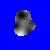
\includegraphics[width=100mm,height=100mm]{figs/hare}
      \caption{This figure shows one of the output files created during a simulation using a $100 \times 100$ grid and default initial conditions. Various shades of grey represent the density of hares after 50 time steps, with a time step set to 0.4.}
      \end{center}
      \end{figure}
      
     % \newline{}
      The number of the *.ppm files created depends on the initial parameters specified by the user, $dt$ and $T$. To maximise the level of output clarity we decided to make separate landscape "maps" for each type of animal, here pumas and hares. In each "map" the pixels corresponding to water cells are shown in blue, while the land cells are white. The variation in density of pumas/hares across the land cells is represented by different shades of grey, with black colour corresponding to the maximum value. 
      \newline{}
      For each type of animal, every $T$ time steps, the code also calculates the mean population density and writes it along with the corresponding time into a file. 
      

      
      	
      
      
      \subsection{GUI} %dmitry
GUIs are not used in HPC as they use memory and slow down computations and are generally not necessary as all the interactions with HPC machines is done through a command line.
However, our group has chosen to code in Java, and GUI is one of Java's strengths as it should look the same on every machine. So it was decided that we are not taking advantages of our chosen language unless we create a GUI. 
GUI created is responsible for the input parameters of the simulation. Initially, it would just take the values and run the simulation.
\begin{figure} [BeforeRange]
\begin{center}
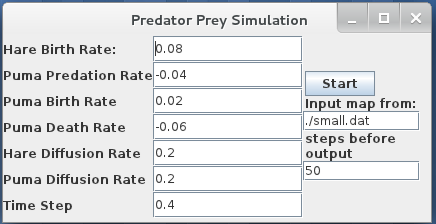
\includegraphics[scale = 0.5]{figs/BeforeRange.png}
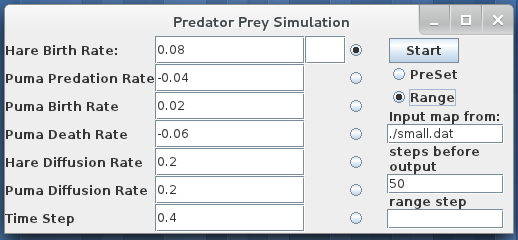
\includegraphics[scale = 0.47]{figs/WithRange.png}
\caption{GUI: Initial version and final version}
\label{fig:BeforeRange}
\end{center}
\end{figure}
However, in later) versions, \emph{range} option was added to be able to run multiple simulations changing one of the parameters (see fig. \ref{fig:BeforeRange}).
The frame is divided into three parts (all on separate frames): input, input2, button (see fig. \ref{fig:input}).
Input holds labels and text fields for parameter inputs. 
\begin{figure} [input]
\begin{center}
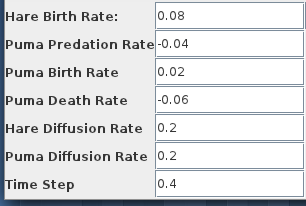
\includegraphics[scale = 0.5]{figs/input.png}
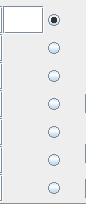
\includegraphics[scale = 0.5]{figs/input2.png}
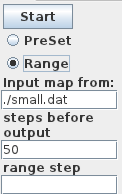
\includegraphics[scale = 0.5]{figs/button.png}
\caption{Panels: input, input2, button}
\label{fig:input}
\end{center}
\end{figure}
Input2 holds second text field and radio buttons to chose which parameter to range over, is not visible unless range is selected. 
Button holds start button, choice between range and preset values and parameter values that are general like input file, steps before output.
Gui is still very simplistic and could be enhanced more but was not due to time constraints
   
   \section{Tools}
   %matt
Most of the group members (DID WE ALL USE ECLIPSE?) used the Eclipse IDE to develop the program. Eclipse provides many useful features that aid the development process including an extensive debugger, realtime error checking, comprehensive autocompleting and support for JUnit testing. In addition to Eclipse a number of other tools were utilised, details of which can be found in the following sections.
      \subsection{SVN} %matt
	We chose to host the SVN repository using a Google Code project. The home page can be found at \href{http://code.google.com/p/ps-predator-prey/}{http://code.google.com/p/ps-predator-prey/}. Doing so allowed us to make use of the many excellent tools that are available for managing such projects; the most obvious example being the ability to quickly and easily browse all of the revisions from r1 current via the web interface.  The fact that the code was hosted externally on a 24/h server meant that it could be accessed from anywhere at any time. There was also no issue with compatibility: Some of the group members opted to use the SVN Eclipse plug that interfaces seamlessly with the Google Code while others chose to use the more traditional approach of checking code in and out via the command line. Another invaluable feature was the ability to compare side by side any and all changes between revisions. See for example the changes made to Output.java in revision r29:\\* \\*
	 \href{http://code.google.com/p/ps-predator-prey/source/diff?spec=svn29&r=29&format=side&path=/code/Output.java}{http://code.google.com/p/ps-predator-prey/source/diff?spec=svn29&r=29&format=side&path=/code/Output.java} \\* \\*
	 This feature is compatible with all text files, and so also proved useful for the group editing of latex files.	      
      
      \subsection{Ant File} %tom, Jorge 
To automate the building of the software, we have coded an Ant file using the XML language. The Ant file contains the appropriate sections that ensures compilation uses the correct files in the right packages. In order to maintain portability, we included a lib/ directory that contains libraries necessary to the Ant program, so it needs not search the local file system. The scripts also produces a .jar file containing the whole project for easy transportation.  
 
      \subsection{Unit Testing} %jorge
      Every class of the project form a functional unit according to the design elaborated at the beginning of the project. In order to ensure the software's good functioning and correct behaviour, all classes have been tested using the Java JUnit framework with test cases to tackle programming errors and code bugs.

The libraries necessary to the tests are thus accessed from the test cases using Java import statements and extending the TestCase superclass in the class declaration:
\begin{lstlisting}[language=Java,caption= Test case headers]
import org.junit.Before;
import org.junit.Test;
import junit.framework.TestCase;

public class TestAnimal extends TestCase {
...
\end{lstlisting}

The test cases, for each class, follow the normal directives in use for Unit testing with JUnit. The most relevant methods were submitted to thorough tests, where their properties, return values and correct functioning were evaluated by comparing the actual results they provide with the expected ones. These procedures were implemented by test methods in each test case using the format required by the JUnit standards. 

Every test case includes a setup() method that builds the initial object and its different parameters. Directives like @Before and @Test for every method declaration were thus inserted in the code were appropriate. The functioning of a method is then assessed comparing the expected results with the actual ones with JUnit testing methods such as AssertEquals(), AssertNotNull(), etc...

\begin{lstlisting}[language=Java,caption= Use of JUnit directives in test cases]
@Before
public void setUp() {
    ...
    testAnimal = new Animal(numbAnimals);
    testAnimal.setName("Puma");
    ...
@Test
public void testAnimal() {
    assertNotNull(testAnimal);
    assertNotNull(testAnimal2);
} 
...
\end{lstlisting}

Where possible and where the tests were failing, we corrected and bettered the code until all tests passed correctly. We have employed several different methods and tools to debug the code, mainly with Eclipse IDE's debugger and JDB (Java Debugger) at the command line, that enabled us to verify the variables in use in classes and methods are holding the correct desired values during runtime. We have in this manner corrected many mistakes and wrong operations until the software was performing as expected. We also have used certain programming techniques such as Test Driven Development, unfortunately in just a few classes, although the procedure would deserve more time and practice to achieve a reasonable degree of maturity and efficiency to prove a powerful tool. 

\chapter{Results}

	\section{Output Analysis}
	\begin{figure}[h]
   
   % GNUPLOT: LaTeX picture with Postscript
\begingroup
  \makeatletter
  \providecommand\color[2][]{%
    \GenericError{(gnuplot) \space\space\space\@spaces}{%
      Package color not loaded in conjunction with
      terminal option `colourtext'%
    }{See the gnuplot documentation for explanation.%
    }{Either use 'blacktext' in gnuplot or load the package
      color.sty in LaTeX.}%
    \renewcommand\color[2][]{}%
  }%
  \providecommand\includegraphics[2][]{%
    \GenericError{(gnuplot) \space\space\space\@spaces}{%
      Package graphicx or graphics not loaded%
    }{See the gnuplot documentation for explanation.%
    }{The gnuplot epslatex terminal needs graphicx.sty or graphics.sty.}%
    \renewcommand\includegraphics[2][]{}%
  }%
  \providecommand\rotatebox[2]{#2}%
  \@ifundefined{ifGPcolor}{%
    \newif\ifGPcolor
    \GPcolortrue
  }{}%
  \@ifundefined{ifGPblacktext}{%
    \newif\ifGPblacktext
    \GPblacktexttrue
  }{}%
  % define a \g@addto@macro without @ in the name:
  \let\gplgaddtomacro\g@addto@macro
  % define empty templates for all commands taking text:
  \gdef\gplbacktext{}%
  \gdef\gplfronttext{}%
  \makeatother
  \ifGPblacktext
    % no textcolor at all
    \def\colorrgb#1{}%
    \def\colorgray#1{}%
  \else
    % gray or color?
    \ifGPcolor
      \def\colorrgb#1{\color[rgb]{#1}}%
      \def\colorgray#1{\color[gray]{#1}}%
      \expandafter\def\csname LTw\endcsname{\color{white}}%
      \expandafter\def\csname LTb\endcsname{\color{black}}%
      \expandafter\def\csname LTa\endcsname{\color{black}}%
      \expandafter\def\csname LT0\endcsname{\color[rgb]{1,0,0}}%
      \expandafter\def\csname LT1\endcsname{\color[rgb]{0,1,0}}%
      \expandafter\def\csname LT2\endcsname{\color[rgb]{0,0,1}}%
      \expandafter\def\csname LT3\endcsname{\color[rgb]{1,0,1}}%
      \expandafter\def\csname LT4\endcsname{\color[rgb]{0,1,1}}%
      \expandafter\def\csname LT5\endcsname{\color[rgb]{1,1,0}}%
      \expandafter\def\csname LT6\endcsname{\color[rgb]{0,0,0}}%
      \expandafter\def\csname LT7\endcsname{\color[rgb]{1,0.3,0}}%
      \expandafter\def\csname LT8\endcsname{\color[rgb]{0.5,0.5,0.5}}%
    \else
      % gray
      \def\colorrgb#1{\color{black}}%
      \def\colorgray#1{\color[gray]{#1}}%
      \expandafter\def\csname LTw\endcsname{\color{white}}%
      \expandafter\def\csname LTb\endcsname{\color{black}}%
      \expandafter\def\csname LTa\endcsname{\color{black}}%
      \expandafter\def\csname LT0\endcsname{\color{black}}%
      \expandafter\def\csname LT1\endcsname{\color{black}}%
      \expandafter\def\csname LT2\endcsname{\color{black}}%
      \expandafter\def\csname LT3\endcsname{\color{black}}%
      \expandafter\def\csname LT4\endcsname{\color{black}}%
      \expandafter\def\csname LT5\endcsname{\color{black}}%
      \expandafter\def\csname LT6\endcsname{\color{black}}%
      \expandafter\def\csname LT7\endcsname{\color{black}}%
      \expandafter\def\csname LT8\endcsname{\color{black}}%
    \fi
  \fi
  \setlength{\unitlength}{0.0500bp}%
  \begin{picture}(7200.00,5040.00)%
    \gplgaddtomacro\gplbacktext{%
      \csname LTb\endcsname%
      \put(860,640){\makebox(0,0)[r]{\strut{} 0}}%
      \put(860,1400){\makebox(0,0)[r]{\strut{} 1}}%
      \put(860,2160){\makebox(0,0)[r]{\strut{} 2}}%
      \put(860,2920){\makebox(0,0)[r]{\strut{} 3}}%
      \put(860,3680){\makebox(0,0)[r]{\strut{} 4}}%
      \put(860,4440){\makebox(0,0)[r]{\strut{} 5}}%
      \put(980,440){\makebox(0,0){\strut{} 0}}%
      \put(2164,440){\makebox(0,0){\strut{} 100}}%
      \put(3348,440){\makebox(0,0){\strut{} 200}}%
      \put(4532,440){\makebox(0,0){\strut{} 300}}%
      \put(5716,440){\makebox(0,0){\strut{} 400}}%
      \put(6900,440){\makebox(0,0){\strut{} 500}}%
      \put(400,2540){\rotatebox{90}{\makebox(0,0){\strut{}Density}}}%
      \put(3940,140){\makebox(0,0){\strut{}Time [s]}}%
      \put(3940,4740){\makebox(0,0){\strut{}Population Density vs. Time}}%
    }%
    \gplgaddtomacro\gplfronttext{%
      \csname LTb\endcsname%
      \put(5997,4277){\makebox(0,0)[r]{\strut{}Hares}}%
      \csname LTb\endcsname%
      \put(5997,4077){\makebox(0,0)[r]{\strut{}Pumas}}%
    }%
    \gplbacktext
    \put(0,0){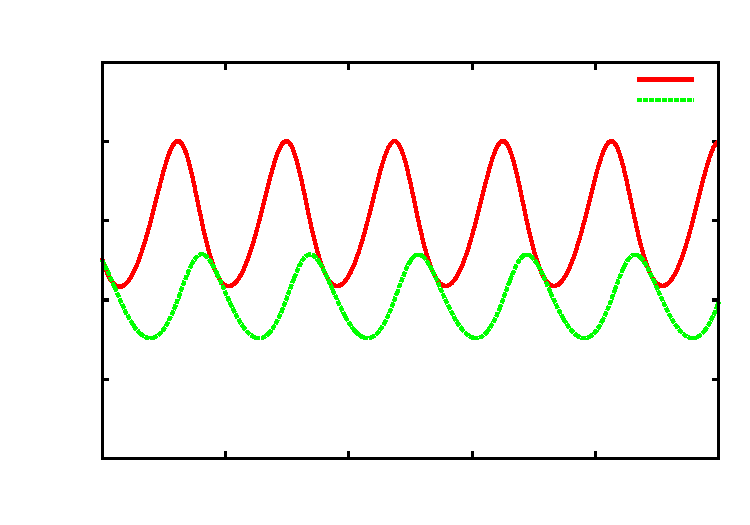
\includegraphics{figs/density}}%
    \gplfronttext
  \end{picture}%
\endgroup

   \caption{Population density vs. time for Hares and Pumas. This periodic behaviour is typical of predator-prey interactions.}
   \end{figure}

   \section{Performance Analysis} %chen+tom
   
    Because most optimisation in Java is done at runtime using Just-In-Time (JIT) compilation, there is not much to choose from in the way
  	 of compiler flags. The way in which a problem is laid out is always very important, however, so our main aim in performance testing
 	 was to identify inefficiencies within the code itself, such as unnecessary loops and calls to methods.\newline{}
 	
 	 Profiling of the code was done mostly with NetBeans and the unix \emph{time} command. Parameters were varied to asses the effect of a number of 
 	 factors, most notably overhead, output write time, and the effect of map size and complexity.\newline{}
 
 	 One of the main things which we identified	very quickly as a bottleneck was the output . Fortunately, implementing a bufered writer is
	 very easy in Java; this alone increased performance by a factor of 5-6 (see Figure \ref{buffering}).\newline{}
	 
	The performance of the program could be increased even further by having the output in a more efficient format. This can be shown more 
   simply by running the code with an output frequency of 50 timesteps compared with an output frequency of 5000 timesteps (a single output for a t=0..500, timestep=0.4
   simulation). This give run times of $\sim$21.5 and $\sim$17.0 seconds respectively, even with buffered output. This output then accounts for 
   $\sim$ 17\% of the computation time of a simulation, which is obviously not ideal.  \newline{}

	
  \begin{figure}[H]
  \begin{center}
  % GNUPLOT: LaTeX picture with Postscript
\begingroup
  \makeatletter
  \providecommand\color[2][]{%
    \GenericError{(gnuplot) \space\space\space\@spaces}{%
      Package color not loaded in conjunction with
      terminal option `colourtext'%
    }{See the gnuplot documentation for explanation.%
    }{Either use 'blacktext' in gnuplot or load the package
      color.sty in LaTeX.}%
    \renewcommand\color[2][]{}%
  }%
  \providecommand\includegraphics[2][]{%
    \GenericError{(gnuplot) \space\space\space\@spaces}{%
      Package graphicx or graphics not loaded%
    }{See the gnuplot documentation for explanation.%
    }{The gnuplot epslatex terminal needs graphicx.sty or graphics.sty.}%
    \renewcommand\includegraphics[2][]{}%
  }%
  \providecommand\rotatebox[2]{#2}%
  \@ifundefined{ifGPcolor}{%
    \newif\ifGPcolor
    \GPcolortrue
  }{}%
  \@ifundefined{ifGPblacktext}{%
    \newif\ifGPblacktext
    \GPblacktexttrue
  }{}%
  % define a \g@addto@macro without @ in the name:
  \let\gplgaddtomacro\g@addto@macro
  % define empty templates for all commands taking text:
  \gdef\gplbacktext{}%
  \gdef\gplfronttext{}%
  \makeatother
  \ifGPblacktext
    % no textcolor at all
    \def\colorrgb#1{}%
    \def\colorgray#1{}%
  \else
    % gray or color?
    \ifGPcolor
      \def\colorrgb#1{\color[rgb]{#1}}%
      \def\colorgray#1{\color[gray]{#1}}%
      \expandafter\def\csname LTw\endcsname{\color{white}}%
      \expandafter\def\csname LTb\endcsname{\color{black}}%
      \expandafter\def\csname LTa\endcsname{\color{black}}%
      \expandafter\def\csname LT0\endcsname{\color[rgb]{1,0,0}}%
      \expandafter\def\csname LT1\endcsname{\color[rgb]{0,1,0}}%
      \expandafter\def\csname LT2\endcsname{\color[rgb]{0,0,1}}%
      \expandafter\def\csname LT3\endcsname{\color[rgb]{1,0,1}}%
      \expandafter\def\csname LT4\endcsname{\color[rgb]{0,1,1}}%
      \expandafter\def\csname LT5\endcsname{\color[rgb]{1,1,0}}%
      \expandafter\def\csname LT6\endcsname{\color[rgb]{0,0,0}}%
      \expandafter\def\csname LT7\endcsname{\color[rgb]{1,0.3,0}}%
      \expandafter\def\csname LT8\endcsname{\color[rgb]{0.5,0.5,0.5}}%
    \else
      % gray
      \def\colorrgb#1{\color{black}}%
      \def\colorgray#1{\color[gray]{#1}}%
      \expandafter\def\csname LTw\endcsname{\color{white}}%
      \expandafter\def\csname LTb\endcsname{\color{black}}%
      \expandafter\def\csname LTa\endcsname{\color{black}}%
      \expandafter\def\csname LT0\endcsname{\color{black}}%
      \expandafter\def\csname LT1\endcsname{\color{black}}%
      \expandafter\def\csname LT2\endcsname{\color{black}}%
      \expandafter\def\csname LT3\endcsname{\color{black}}%
      \expandafter\def\csname LT4\endcsname{\color{black}}%
      \expandafter\def\csname LT5\endcsname{\color{black}}%
      \expandafter\def\csname LT6\endcsname{\color{black}}%
      \expandafter\def\csname LT7\endcsname{\color{black}}%
      \expandafter\def\csname LT8\endcsname{\color{black}}%
    \fi
  \fi
  \setlength{\unitlength}{0.0500bp}%
  \begin{picture}(7200.00,4536.00)%
    \gplgaddtomacro\gplbacktext{%
      \csname LTb\endcsname%
      \put(1100,640){\makebox(0,0)[r]{\strut{} 0.2}}%
      \put(1100,1189){\makebox(0,0)[r]{\strut{} 0.4}}%
      \put(1100,1739){\makebox(0,0)[r]{\strut{} 0.6}}%
      \put(1100,2288){\makebox(0,0)[r]{\strut{} 0.8}}%
      \put(1100,2837){\makebox(0,0)[r]{\strut{} 1}}%
      \put(1100,3387){\makebox(0,0)[r]{\strut{} 1.2}}%
      \put(1100,3936){\makebox(0,0)[r]{\strut{} 1.4}}%
      \put(1220,440){\makebox(0,0){\strut{} 0}}%
      \put(2356,440){\makebox(0,0){\strut{} 200}}%
      \put(3492,440){\makebox(0,0){\strut{} 400}}%
      \put(4628,440){\makebox(0,0){\strut{} 600}}%
      \put(5764,440){\makebox(0,0){\strut{} 800}}%
      \put(6900,440){\makebox(0,0){\strut{} 1000}}%
      \put(400,2288){\rotatebox{90}{\makebox(0,0){\strut{}log$_{10}$ Run Time [s]}}}%
      \put(4060,140){\makebox(0,0){\strut{}Output Frequency (Timesteps)}}%
      \put(4060,4236){\makebox(0,0){\strut{}Effect of Buffered File Writing}}%
    }%
    \gplgaddtomacro\gplfronttext{%
      \csname LTb\endcsname%
      \put(5997,3773){\makebox(0,0)[r]{\strut{}100x100 Buffered}}%
      \csname LTb\endcsname%
      \put(5997,3573){\makebox(0,0)[r]{\strut{}100x100 Unbuffered}}%
    }%
    \gplbacktext
    \put(0,0){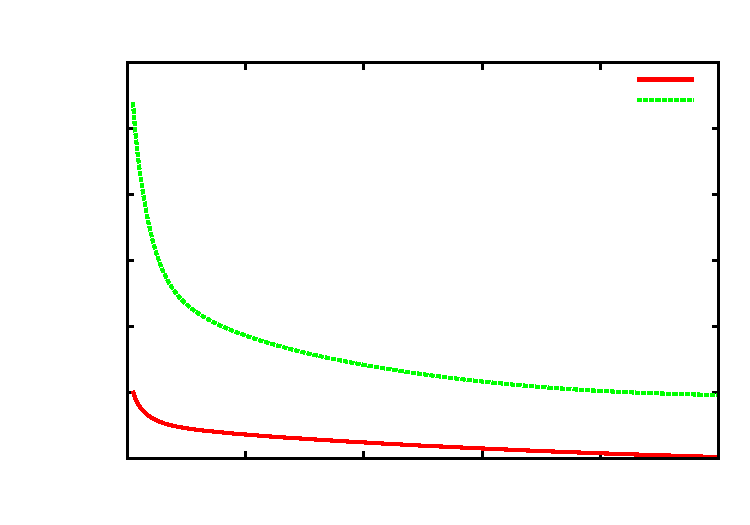
\includegraphics{figs/buffering}}%
    \gplfronttext
  \end{picture}%
\endgroup

  \caption{\label{buffering}This graph shows the advantage of using a buffered file writer over repeated calls to the printf() method. 
  The data was generated from a simulation using a 100x100 grid, but results will be similar for all grid sizes, since write time and computation
  time (neglecting overhead) both scale linearly with the number of cells.}
  \end{center}
  \end{figure} 

	 In Figure \ref{overhead} we attempt to quantify the overhead in our code. This is done by calculating the total time spent on each cell in a 
	 simulation, relative to the size of the simulation. With this metric, the code actually becomes `slower' for smaller simulations. This is 
	 because a significant fraction of the simulation time is being spent on finding arrays of neighbours and other `non essential' tasks. The graph
	 shows that our code only begins to run as efficiently as possible once grids of $\sim$100x100 are used, above which the simulation time scales
	 almost exactly as the number of cells (the flat part of Figure \ref{overhead}).\newline{}

	 
	 It can be seen from Figure \ref{overhead} that, for large simulations, the total time per cell per timestep is constant. The value on the 
	 graph is roughly -3.27, although this is total time per cell. Thus, $10^{-3.27}/1200$, where 1200 is the number of timesteps, gives us the 
	 time per cell per timestep: $\sim$450 nanoseconds.
	 
  \begin{figure}[H]
  \begin{center}
  % GNUPLOT: LaTeX picture with Postscript
\begingroup
  \makeatletter
  \providecommand\color[2][]{%
    \GenericError{(gnuplot) \space\space\space\@spaces}{%
      Package color not loaded in conjunction with
      terminal option `colourtext'%
    }{See the gnuplot documentation for explanation.%
    }{Either use 'blacktext' in gnuplot or load the package
      color.sty in LaTeX.}%
    \renewcommand\color[2][]{}%
  }%
  \providecommand\includegraphics[2][]{%
    \GenericError{(gnuplot) \space\space\space\@spaces}{%
      Package graphicx or graphics not loaded%
    }{See the gnuplot documentation for explanation.%
    }{The gnuplot epslatex terminal needs graphicx.sty or graphics.sty.}%
    \renewcommand\includegraphics[2][]{}%
  }%
  \providecommand\rotatebox[2]{#2}%
  \@ifundefined{ifGPcolor}{%
    \newif\ifGPcolor
    \GPcolortrue
  }{}%
  \@ifundefined{ifGPblacktext}{%
    \newif\ifGPblacktext
    \GPblacktexttrue
  }{}%
  % define a \g@addto@macro without @ in the name:
  \let\gplgaddtomacro\g@addto@macro
  % define empty templates for all commands taking text:
  \gdef\gplbacktext{}%
  \gdef\gplfronttext{}%
  \makeatother
  \ifGPblacktext
    % no textcolor at all
    \def\colorrgb#1{}%
    \def\colorgray#1{}%
  \else
    % gray or color?
    \ifGPcolor
      \def\colorrgb#1{\color[rgb]{#1}}%
      \def\colorgray#1{\color[gray]{#1}}%
      \expandafter\def\csname LTw\endcsname{\color{white}}%
      \expandafter\def\csname LTb\endcsname{\color{black}}%
      \expandafter\def\csname LTa\endcsname{\color{black}}%
      \expandafter\def\csname LT0\endcsname{\color[rgb]{1,0,0}}%
      \expandafter\def\csname LT1\endcsname{\color[rgb]{0,1,0}}%
      \expandafter\def\csname LT2\endcsname{\color[rgb]{0,0,1}}%
      \expandafter\def\csname LT3\endcsname{\color[rgb]{1,0,1}}%
      \expandafter\def\csname LT4\endcsname{\color[rgb]{0,1,1}}%
      \expandafter\def\csname LT5\endcsname{\color[rgb]{1,1,0}}%
      \expandafter\def\csname LT6\endcsname{\color[rgb]{0,0,0}}%
      \expandafter\def\csname LT7\endcsname{\color[rgb]{1,0.3,0}}%
      \expandafter\def\csname LT8\endcsname{\color[rgb]{0.5,0.5,0.5}}%
    \else
      % gray
      \def\colorrgb#1{\color{black}}%
      \def\colorgray#1{\color[gray]{#1}}%
      \expandafter\def\csname LTw\endcsname{\color{white}}%
      \expandafter\def\csname LTb\endcsname{\color{black}}%
      \expandafter\def\csname LTa\endcsname{\color{black}}%
      \expandafter\def\csname LT0\endcsname{\color{black}}%
      \expandafter\def\csname LT1\endcsname{\color{black}}%
      \expandafter\def\csname LT2\endcsname{\color{black}}%
      \expandafter\def\csname LT3\endcsname{\color{black}}%
      \expandafter\def\csname LT4\endcsname{\color{black}}%
      \expandafter\def\csname LT5\endcsname{\color{black}}%
      \expandafter\def\csname LT6\endcsname{\color{black}}%
      \expandafter\def\csname LT7\endcsname{\color{black}}%
      \expandafter\def\csname LT8\endcsname{\color{black}}%
    \fi
  \fi
  \setlength{\unitlength}{0.0500bp}%
  \begin{picture}(7200.00,4536.00)%
    \gplgaddtomacro\gplbacktext{%
      \csname LTb\endcsname%
      \put(1100,640){\makebox(0,0)[r]{\strut{}-3.5}}%
      \put(1100,1111){\makebox(0,0)[r]{\strut{}-3.0}}%
      \put(1100,1582){\makebox(0,0)[r]{\strut{}-2.5}}%
      \put(1100,2053){\makebox(0,0)[r]{\strut{}-2.0}}%
      \put(1100,2523){\makebox(0,0)[r]{\strut{}-1.5}}%
      \put(1100,2994){\makebox(0,0)[r]{\strut{}-1.0}}%
      \put(1100,3465){\makebox(0,0)[r]{\strut{}-0.5}}%
      \put(1100,3936){\makebox(0,0)[r]{\strut{} 0.0}}%
      \put(1220,440){\makebox(0,0){\strut{} 0}}%
      \put(2167,440){\makebox(0,0){\strut{} 1}}%
      \put(3113,440){\makebox(0,0){\strut{} 2}}%
      \put(4060,440){\makebox(0,0){\strut{} 3}}%
      \put(5007,440){\makebox(0,0){\strut{} 4}}%
      \put(5953,440){\makebox(0,0){\strut{} 5}}%
      \put(6900,440){\makebox(0,0){\strut{} 6}}%
      \put(400,2288){\rotatebox{90}{\makebox(0,0){\strut{}log$_{10}$ Time/Cell [s]}}}%
      \put(4060,140){\makebox(0,0){\strut{}log$_{10}$ Number of Cells}}%
      \put(4060,4236){\makebox(0,0){\strut{}Run Time/Number of Cells vs. Number of Cells}}%
    }%
    \gplgaddtomacro\gplfronttext{%
      \csname LTb\endcsname%
      \put(5997,3773){\makebox(0,0)[r]{\strut{}Run Time/Number of Cells}}%
    }%
    \gplbacktext
    \put(0,0){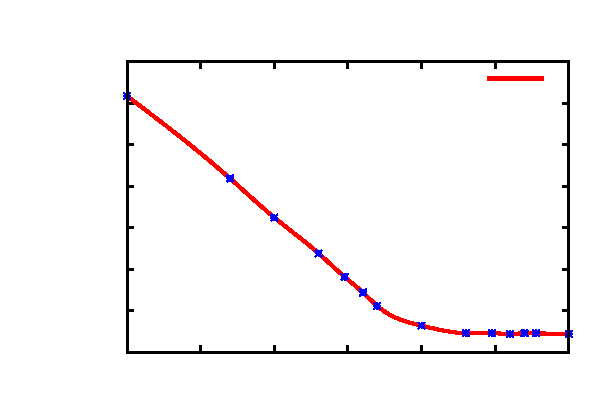
\includegraphics{figs/overhead}}%
    \gplfronttext
  \end{picture}%
\endgroup

  \caption{\label{overhead}This is a graph of total time spent on each cell, which shows that overheads such as array initialization
  take up a significant fraction of computation time with grids smaller than $\sim$100 by 100.}
  \end{center}
  \end{figure}
  
  \begin{figure}[H]
  \begin{center}
  \subfloat[]{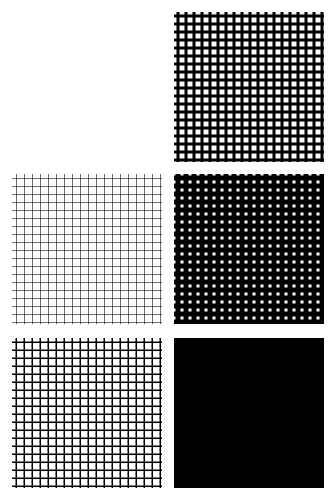
\includegraphics[width=40mm]{figs/emptypic.png}}
  \subfloat[]{% GNUPLOT: LaTeX picture with Postscript
\begingroup
  \makeatletter
  \providecommand\color[2][]{%
    \GenericError{(gnuplot) \space\space\space\@spaces}{%
      Package color not loaded in conjunction with
      terminal option `colourtext'%
    }{See the gnuplot documentation for explanation.%
    }{Either use 'blacktext' in gnuplot or load the package
      color.sty in LaTeX.}%
    \renewcommand\color[2][]{}%
  }%
  \providecommand\includegraphics[2][]{%
    \GenericError{(gnuplot) \space\space\space\@spaces}{%
      Package graphicx or graphics not loaded%
    }{See the gnuplot documentation for explanation.%
    }{The gnuplot epslatex terminal needs graphicx.sty or graphics.sty.}%
    \renewcommand\includegraphics[2][]{}%
  }%
  \providecommand\rotatebox[2]{#2}%
  \@ifundefined{ifGPcolor}{%
    \newif\ifGPcolor
    \GPcolortrue
  }{}%
  \@ifundefined{ifGPblacktext}{%
    \newif\ifGPblacktext
    \GPblacktexttrue
  }{}%
  % define a \g@addto@macro without @ in the name:
  \let\gplgaddtomacro\g@addto@macro
  % define empty templates for all commands taking text:
  \gdef\gplbacktext{}%
  \gdef\gplfronttext{}%
  \makeatother
  \ifGPblacktext
    % no textcolor at all
    \def\colorrgb#1{}%
    \def\colorgray#1{}%
  \else
    % gray or color?
    \ifGPcolor
      \def\colorrgb#1{\color[rgb]{#1}}%
      \def\colorgray#1{\color[gray]{#1}}%
      \expandafter\def\csname LTw\endcsname{\color{white}}%
      \expandafter\def\csname LTb\endcsname{\color{black}}%
      \expandafter\def\csname LTa\endcsname{\color{black}}%
      \expandafter\def\csname LT0\endcsname{\color[rgb]{1,0,0}}%
      \expandafter\def\csname LT1\endcsname{\color[rgb]{0,1,0}}%
      \expandafter\def\csname LT2\endcsname{\color[rgb]{0,0,1}}%
      \expandafter\def\csname LT3\endcsname{\color[rgb]{1,0,1}}%
      \expandafter\def\csname LT4\endcsname{\color[rgb]{0,1,1}}%
      \expandafter\def\csname LT5\endcsname{\color[rgb]{1,1,0}}%
      \expandafter\def\csname LT6\endcsname{\color[rgb]{0,0,0}}%
      \expandafter\def\csname LT7\endcsname{\color[rgb]{1,0.3,0}}%
      \expandafter\def\csname LT8\endcsname{\color[rgb]{0.5,0.5,0.5}}%
    \else
      % gray
      \def\colorrgb#1{\color{black}}%
      \def\colorgray#1{\color[gray]{#1}}%
      \expandafter\def\csname LTw\endcsname{\color{white}}%
      \expandafter\def\csname LTb\endcsname{\color{black}}%
      \expandafter\def\csname LTa\endcsname{\color{black}}%
      \expandafter\def\csname LT0\endcsname{\color{black}}%
      \expandafter\def\csname LT1\endcsname{\color{black}}%
      \expandafter\def\csname LT2\endcsname{\color{black}}%
      \expandafter\def\csname LT3\endcsname{\color{black}}%
      \expandafter\def\csname LT4\endcsname{\color{black}}%
      \expandafter\def\csname LT5\endcsname{\color{black}}%
      \expandafter\def\csname LT6\endcsname{\color{black}}%
      \expandafter\def\csname LT7\endcsname{\color{black}}%
      \expandafter\def\csname LT8\endcsname{\color{black}}%
    \fi
  \fi
  \setlength{\unitlength}{0.0500bp}%
  \begin{picture}(3600.00,3528.00)%
    \gplgaddtomacro\gplbacktext{%
      \csname LTb\endcsname%
      \put(980,640){\makebox(0,0)[r]{\strut{} 0}}%
      \put(980,1170){\makebox(0,0)[r]{\strut{} 5}}%
      \put(980,1699){\makebox(0,0)[r]{\strut{} 10}}%
      \put(980,2229){\makebox(0,0)[r]{\strut{} 15}}%
      \put(980,2758){\makebox(0,0)[r]{\strut{} 20}}%
      \put(980,3288){\makebox(0,0)[r]{\strut{} 25}}%
      \put(1633,440){\makebox(0,0){\strut{}25}}%
      \put(2189,440){\makebox(0,0){\strut{}50}}%
      \put(2744,440){\makebox(0,0){\strut{}75}}%
      \put(3300,440){\makebox(0,0){\strut{}100}}%
      \put(400,1964){\rotatebox{90}{\makebox(0,0){\strut{}Run Time [s]}}}%
      \put(2200,140){\makebox(0,0){\strut{}Land Percentage}}%
    }%
    \gplgaddtomacro\gplfronttext{%
    }%
    \gplbacktext
    \put(0,0){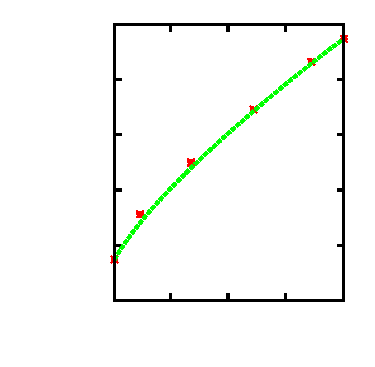
\includegraphics{figs/empty}}%
    \gplfronttext
  \end{picture}%
\endgroup
}
  \caption{\label{empty}This shows the effect of fill percentage on run time. The six panels in a) are the input maps used, all of which were
  300x300. As expected, the computation time increases fairly linearly with
  the amount of land, since the bulk of the main algorithm is only run for land cells.}
  \end{center}
  \end{figure}
  
  


\chapter{Conclusions} %everyone

	The Google Code SNV combined with the ability to compile and run Java code on any platform provided a universal code base that could be accessed from anywhere at any time.    

\end{document}
